\documentclass[pdftex,12pt,a4paper]{article}
\usepackage[pdftex]{graphicx}
\newcommand{\HRule}{\rule{\linewidth}{0.5mm}}
\usepackage{lipsum}
%\usepackage[utf8]{inputenc}
\usepackage[a4paper,margin=2.5cm]{geometry}  
\usepackage{graphicx}% allows you to import images
\usepackage{caption}
\usepackage{subcaption}
\usepackage{float}
\usepackage{wallpaper}

\usepackage[hidelinks]{hyperref}  
%\usepackage{enumitem}
\usepackage{enumerate}
\usepackage{listings}
\usepackage{xcolor}
\usepackage{lipsum}
\usepackage{lmodern}
\usepackage{tcolorbox}
\usepackage{setspace}
\renewcommand{\baselinestretch}{1.1}
%bullet preamlbe
\renewcommand{\labelitemi}{$\bullet$}
\renewcommand{\labelitemii}{$\diamond$}
\renewcommand{\labelitemiii}{$\circle$}
\renewcommand\thesection{\Roman{section}} 
\usepackage{mhchem} % allow us to write chemistry equation
%\usepackage{xfrac}  % allow for slanted fractions
%\usepackage{amsmath}
\usepackage{amssymb}
\usepackage{wasysym}
\usepackage{pifont}
\usepackage{multirow}
\usepackage[makeroom]{cancel}
\usepackage[numbers]{natbib}
\bibliographystyle{unsrt}
\citestyle{IEEEtran}

% shortcut
\def\be{\begin{equation}}
\def\ee{\end{equation}}
\def\bd{\begin{displaymath}}
\def\ed{\end{displaymath}}
\def\bi{\begin{itemize}}
\def\ei{\end{itemize}}
\def\bn{\begin{enumerate}}
\def\en{\end{enumerate}}
\def\ba{\begin{eqnarray*}}
\def\ea{\end{eqnarray*}}
\def\u{\text}  
\def\v{\mathbf}   
\def\^{\textsuperscript}
\def\_{\textsubscript}
\def\inf{\infty}
\def\bf{\textbf}
\lstset{language=Matlab}
\lstset{breaklines}
\lstset{extendedchars=false}


\usepackage{fancyhdr}
\pagestyle{fancy}
\rhead{Group x}
\lhead{ELEN90062}

\begin{document}
\graphicspath{{./figs/}}
\begin{titlepage}
\begin{center}
% Upper part of the page
\begin{figure}[H]
      
\includegraphics[width=6cm]{logo.png}
    \end{figure}
	
	
	%------------------------------------------------
	%	Title
	%------------------------------------------------
	{\color[RGB]{0,0,128} {\huge University of Melbourne}\\[0.5\baselineskip] % Title line 1
		{\Huge ELEN90062 High Speed Electronics  }\\[0.5\baselineskip] % Title line 2
		{\Huge GROUP X}}\\ % Title line 3}}
% Title
\vspace{0.05\textheight} % Whitespace between the rule and authors
\huge \bfseries WORKSHOP 2
\rule{\textwidth}{1pt} % Thick horizontal rule
\vspace{0.02\textheight} % Whitespace between the rule and authors
% Author and supervisor
\begin{flushright} \large
Rui \textsc{YUAN}\\
813927 \\
\end{flushright}
\vfill
% Bottom of the page
\begin{flushright} \large
{\large \today}
\end{flushright}
\rule{\textwidth}{0.4pt} % Thin horizontal rule
	
	\vspace{2pt}\vspace{-\baselineskip} % Whitespace between rules
	
	\rule{\textwidth}{1pt} % Thick horizontal rule
\begin{flushright} \tiny
{\scriptsize  \textcopyright \quad Rui YUAN 2017-2019}
\end{flushright}
\end{center}
\end{titlepage}


\newpage

\section{Colpitts Oscillator Simulation}
\begin{figure}[H]
\centering
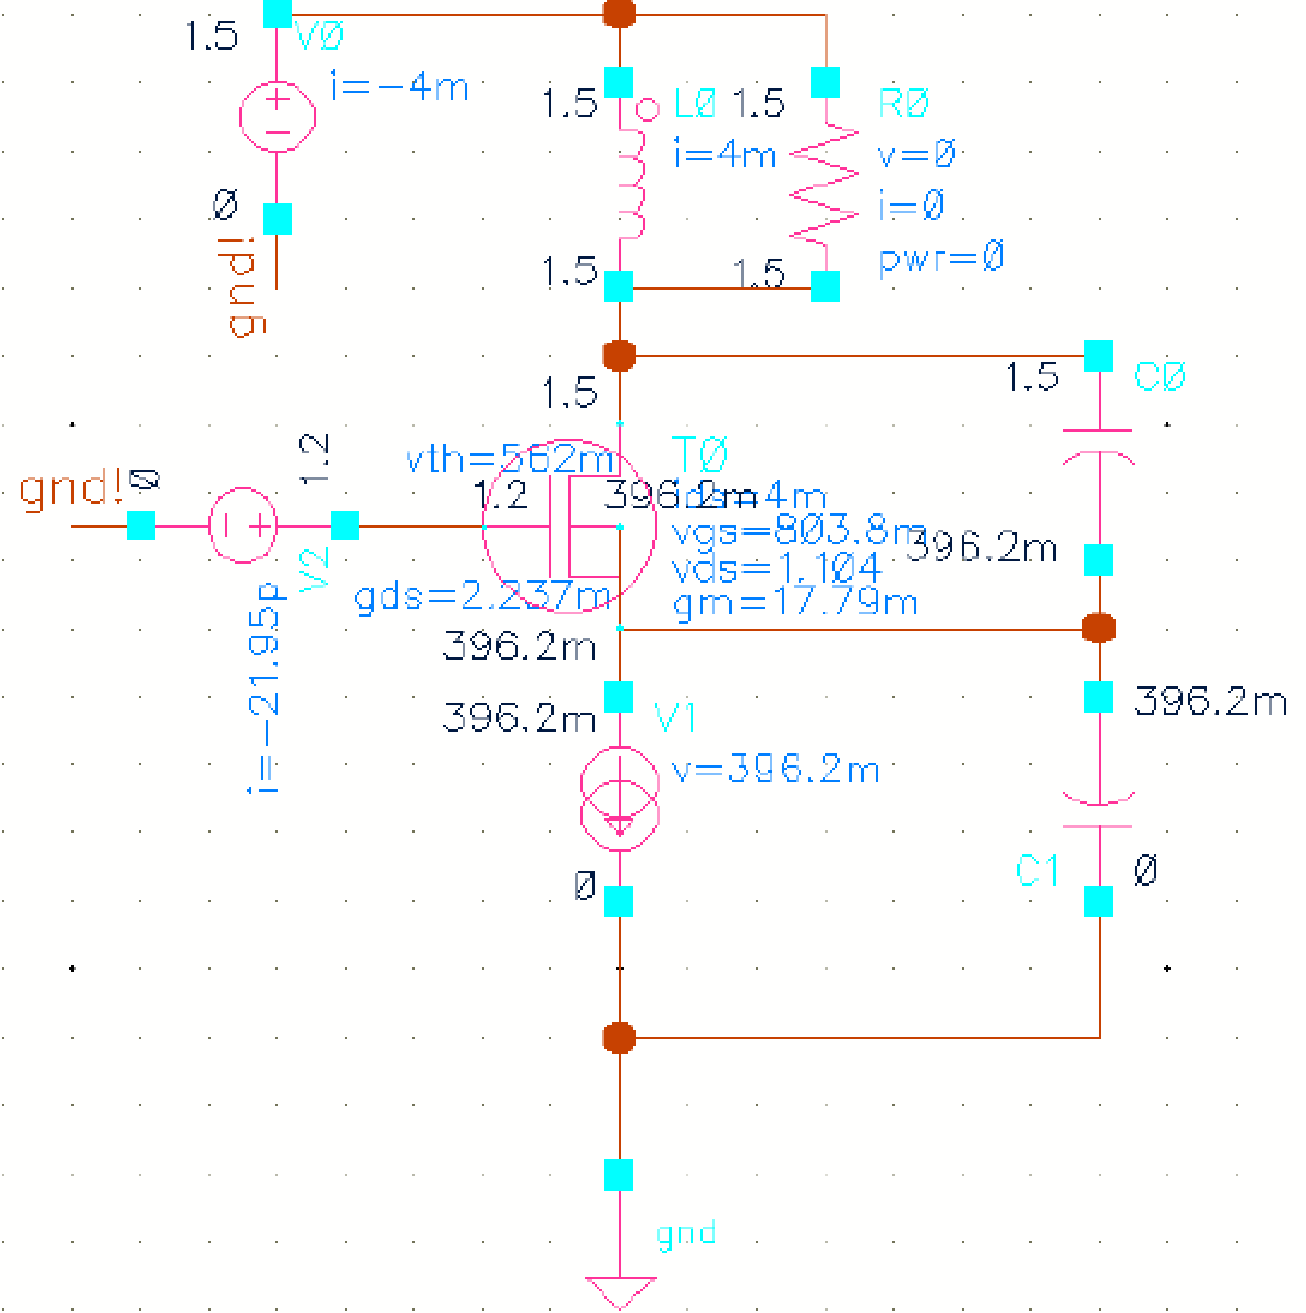
\includegraphics[width=13cm]{ca1.png}
\caption{Schemetic}
\end{figure}
As we are given $L = 1 nH$, $C1 = C2 = 24 pF$, and $R = 500 \Omega$ respectively:
\subsection{Calculate the minimum gain (gm), required to start the oscillations.}
\begin{align}
g_m &>\frac{1}{R(n-n^2)} 
\end{align}
Where:
\begin{align}
n&=\frac{C1}{C1+C2}\\
&=\frac{1}{2}
\end{align}
Hence:
\begin{align}
g_m &>\frac{1}{5000\times(\dfrac{1}{4})}\\
&>0.0008
\end{align}
\subsection{Calculate the frequency of oscillations, f.}
\begin{align}
f&=\frac{1}{2\pi \sqrt{L(\frac{C_1 C_2}{C_1+C_2})}}\\
&=\frac{1}{2\pi \sqrt{1\times 10^{-9}\frac{(24\times 10^{-12})^2}{48\times 10^{-12}}}}\\
&\approx  1.453\times 10^{9}\\
\end{align}
\end{document}